\chapter{Analisis Solusi}

\section{Alternatif Solusi}

Bagian ini membahas alternatif pengoptimalan yang bisa menjadi opsi, tetapi tidak dipilih menjadi bagian dari solusi.

\subsection{Penggunaan \textit{Cache} dengan TTL Kecil}

Meski pada beban tinggi hasil kueri yang di-\textit{cache} akan selalu \textit{stale}, tetap ada durasi hidup (\textit{time to live}) \textit{cache} yang masih dapat diterima. Misalkan, waktu hidup \textit{cache} pembacaan ketersediaan adalah 100-200 milidetik. Rentang waktu ini masih memberikan \textit{data freshness} yang baik dan mampu meminimalkan jumlah kueri yang harus dilakukan sistem. Meskipun begitu, pendekatan ini harus dilakukan pada setiap arsitektur agar perbandingannya setara. Selain itu, pendekatan ini tidak sesuai dengan tujuan tugas akhir ini yang ingin mengoptimalkan operasi baca dan tetap memberikan hasil kueri yang \textit{fresh}.

\subsection{Alternatif Basis Data Terdistribusi}

Selain Citus, terdapat berbagai alternatif basis data terdistribusi lain, seperti Vitess, TiDB, YugabyteDB, dan CockroachDB. Berikut adalah perbandingan masing-masing solusi \parencite{citus,vitess,tiDB,yugabyte,cockroachDB}:

\begingroup
\footnotesize
\begin{longtable}{|p{0.14\textwidth}|p{0.14\textwidth}|p{0.14\textwidth}|p{0.14\textwidth}|p{0.14\textwidth}|p{0.14\textwidth}|}
    \caption{Perbandingan Antara Citus, Vitess, TiDB, YugabyteDB, dan CockroachDB}                                                                                                                                                                                                                    \\
    \hline
    \textbf{Aspek}            & \textbf{Citus}                                               & \textbf{Vitess}                                     & \textbf{TiDB}                                  & \textbf{YugabyteDB}                            & \textbf{CockroachDB}                           \\
    \hline
    \endfirsthead

    \multicolumn{6}{|c|}{\tablename\ \thetable\ -- \textit{Lanjutan dari halaman sebelumnya}}                                                                                                                                                                                                         \\
    \hline
    \textbf{Aspek}            & \textbf{Citus}                                               & \textbf{Vitess}                                     & \textbf{TiDB}                                  & \textbf{YugabyteDB}                            & \textbf{CockroachDB}                           \\
    \hline
    \endhead

    \hline
    \multicolumn{6}{|r|}{\textit{Dilanjutkan ke halaman berikutnya}}                                                                                                                                                                                                                                  \\
    \endfoot

    \hline
    \endlastfoot

    \hline
    Basis data yang mendasari & PostgreSQL                                                   & MySQL                                               & Dibuat dari awal                               & Dibuat dari awal                               & Dibuat dari awal                               \\
    \hline
    \hline
    Arsitektur                & \textit{Sharded Multi-Master with a Coordinator}             & \textit{Sharded Multi-Master with a Coordinator}    & \textit{Multi-Master with Shared Nothing}      & \textit{Multi-Master with Shared Nothing}      & \textit{Multi-Master with Shared Nothing}      \\
    \hline
    \hline
    Tipe                      & Ekstensi PostgreSQL                                          & Ekstensi MySQL                                      & Basis data terdistribusi dengan konsensus Raft & Basis data terdistribusi dengan konsensus Raft & Basis data terdistribusi dengan konsensus Raft \\
    \hline
    \hline
    Kompatibilitas SQL        & PostgreSQL                                                   & MySQL                                               & Kompatibel dengan MySQL 8.0                    & Kompatibel dengan PostgreSQL                   & Kompatibel dengan PostgreSQL                   \\
    \hline
    \hline
    Konsistensi               & Sama seperti PostgreSQL (konsisten dalam satu \textit{node}) & \textit{Eventual consistent} untuk operasi tertentu & ACID                                           & ACID                                           & ACID                                           \\
    \hline
    \hline
    Dukungan CDC              & Ada                                                          & Ada                                                 & Ada                                            & Ada                                            & Ada                                            \\
    \hline
    \hline
    Distribusi Data           & \textit{shard}                                               & \textit{shard}                                      & \textit{native distributed}                    & \textit{native distributed}                    & \textit{native distributed}                    \\
    \hline
\end{longtable}
\endgroup

Distribusi data yang \textit{natively distributed} masih sama-sama berupa \textit{sharding} data. Meskipun begitu, proses \textit{sharding} ini dilakukan secara otomatis dan tidak ditentukan oleh pengguna. Selain itu, suatu \textit{shard} dapat dipegang oleh beberapa \textit{node} sekaligus untuk mencapai \textit{redundancy} dan \textit{fault tolerance}.

Todo kenapa pilih citus selain karena familiarity dengan postgresql dan agar perbandingannya setara dengan arsitektur dasar acuan yang sama-sama menggunakan postgresql

\subsection{Penggunaan Solusi \textit{Serverless}}

Bagaimana dengan solusi serverless?

\section{Arsitektur Solusi}

Setiap arsitektur solusi memiliki dua layanan eksternal, yaitu layanan pengguna dan layanan gerbang pembayaran. Kedua layanan ini akan dibuat \textit{stateless} sehingga penskalaan dapat dilakukan dengan menambah jumlah \textit{instance} layanan. Pada kasus ini, kedua layanan ini akan diusahakan sehingga tidak menjadi sumber \textit{bottleneck}. Layanan pengguna tidak akan menjadi \textit{bottleneck} karena pada saat pengujian akan diasumsikan seluruh pengguna sudah \textit{login} dan pemeriksaan otentikasi dilakukan pada masing-masing \textit{instance backend}.

Komunikasi dengan layanan pembayaran harus dilakukan secara sinkron, setidaknya ketika layanan tiket memanggil layanan pembayaran untuk membuat tagihan. Apabila layanan pembayaran tiket mengalami \textit{bottleneck} pada basis data, pengoptimalan pada basis data akan dilakukan dengan menggunakan kluster Citus sebagaimana yang dilakukan pada arsitektur yang mengoptimalkan PostgreSQL.

\subsection{Arsitektur Dasar Acuan}

\begin{figure}[ht]
    \centering
    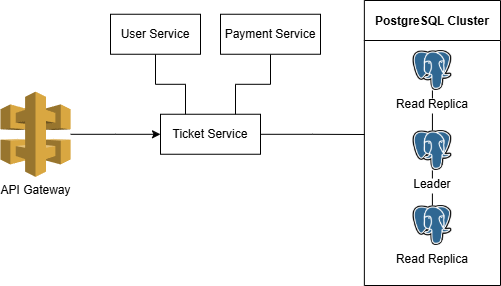
\includegraphics[width=0.8\textwidth]{resources/chapter-3/architecture-reference.png}
    \caption{Arsitektur Dasar Acuan}
    \label{fig:baseline-architecture}
\end{figure}

Arsitektur ini akan menjadi dasar acuan yang digunakan sebagai dasar perbandingan kinerja. Komponen \textit{backend} utama (layanan tiket) bersifat \textit{stateless}, sehingga dapat di-\textit{scale} dengan meningkatkan jumlah \textit{instance}. Kemudian, gerbang API akan melakukan \textit{load balancing} untuk mendistribusikan beban ke beberapa \textit{instance}.

Basis data merupakan komponen yang sulit di-\textit{scale} secara dinamis berdasarkan beban yang diterima. Biasanya, penskalaan secara vertikal merupakan opsi utama untuk meningkatkan \textit{throughput}, terutama dalam operasi tulis. Meskipun begitu, pada arsitektur ini terdapat kluster PostgreSQL dengan konfigurasi satu node pemimpin dan sisanya node replika. Keberadaan replika memungkinkan peningkatan \textit{throughput} permintaan baca, meski tidak ada peningkatan \textit{throughput} untuk operasi tulis.

\subsection{Arsitektur yang Mengoptimalkan PostgreSQL}

\begin{figure}[ht]
    \centering
    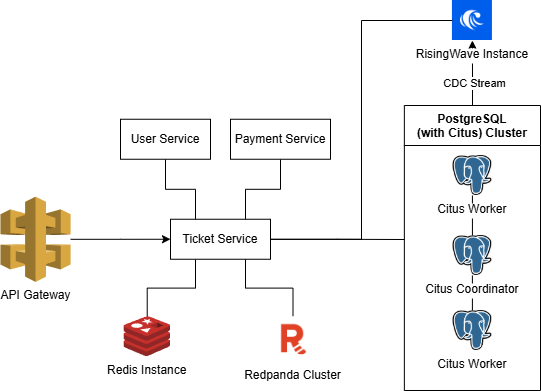
\includegraphics[width=0.8\textwidth]{resources/chapter-3/architecture-optimized.png}
    \caption{Arsitektur yang Mengoptimalkan PostgreSQL}
    \label{fig:optimized-architecture}
\end{figure}

Arsitektur ini mengoptimalkan sistem dengan pola CQRS. Tanggung jawab permintaan baca dilimpahkan kepada RisingWave. \textit{Streaming database} ini mengonsumsi \textit{CDC stream} dari kluster PostgreSQL, lalu memperbarui kueri secara inkremental. Hal yang perlu diperhatikan dalam penggunaan RisingWave adalah \textit{replication lag}. Data yang dikembalikan oleh RisingWave tidak valid apabila data tersebut \textit{outdated}. Penggunaan ekstensi Citus memungkinkan pembagian data berdasarkan baris dan \textit{multiple writer}. Selain itu, perintah pemesanan tiket (berupa \textit{command}/ \textit{event sourcing}) akan dimasukkan ke dalam antrean terlebih dahulu, lalu diproses secara bertahap. Redis digunakan untuk menyimpan \textit{uncommited data} dan menolak permintaan pemesanan lebih awal.

Penggunaan ekstensi Citus memungkinkan peningkatan \textit{write throughput} tidak hanya dengan pendekatan \textit{scale up}, tetapi juga dengan pendekatan \textit{scale-out}. Redpanda dapat dibuat kluster dengan pemartisian data untuk meningkatkan \textit{throughput}.

\textit{Persistence} pada Redis bersifat asinkron, sehingga terdapat kemungkinan data hilang ketika terjadi kegagalan. Meskipun begitu, penggunaan \textit{key-value store} lain yang \textit{persistent} berpotensi memperlambat kinerja. Dalam kasus ini, Redis akan dikonfigurasikan dalam mode kluster untuk redundansi dan mode AOF untuk \textit{persistence}. Hilangnya data hanya akan terjadi ketika \textit{master} dan \textit{replica} mengalami kegagalan dalam satu waktu. Selain itu, hilangnya data pada Redis tidak akan mengganggu integritas data karena pemeriksaan kedua masih akan dilakukan saat pemrosesan data.

\subsection{Arsitektur \textit{Event-Driven}}

\begin{figure}[ht]
    \centering
    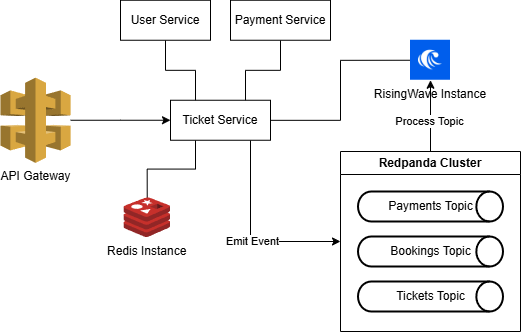
\includegraphics[width=0.8\textwidth]{resources/chapter-3/architecture-event-driven.png}
    \caption{Arsitektur \textit{Event-Driven}}
    \label{fig:solution-event-driven-architecture}
\end{figure}

Arsitektur ini tidak menggunakan PostgreSQL sama sekali. Pada dasarnya, basis data relasional terdiri atas komponen \textit{storage} dan \textit{query processor}. Pada arsitektur ini, komponen \textit{storage} diganti menggunakan Redpanda dengan berbagai topik dan \textit{query processor} diganti dengan RisingWave. Meskipun begitu, pendekatan ini tidak memiliki dukungan \textit{transaction} selain \textit{transaction} pada Redpanda yang berupa \textit{push log all or nothing} pada beberapa topik sekaligus. Untuk itu, Redis digunakan untuk menyimpan \textit{dirty data} atau \textit{uncommited data} sehingga untuk mencegah \textit{double booking}.

Redpanda dapat dibuat kluster dengan pemartisian data untuk meningkatkan \textit{throughput}. Selain itu, RisingWave merupakan \textit{streaming database} yang \textit{cloud-native} sehingga dapat di-\textit{scale out} dengan mudah untuk meningkatkan \textit{throughput}.

Isu \textit{persistence} Redis pada arsitektur ini lebih penting daripada arsitektur sebelumnya. Meskipun begitu, penggunaan kluster dan mode AOF masih dianggap cukup dengan konfigurasi tambahan. Untuk menjamin \textit{stronger durability}, Redis akan dikonfigurasikan untuk selalu melakukan penulisan langsung setelah perintah dijalankan (\texttt{appendfsync always}). Konfigurasi ini akan melakukan penulisan langsung setelah perintah dijalankan. Berbeda dengan konfigurasi \textit{default} Redis yang baru melakukan operasi tulis setiap detik. Kluster Redis masih digunakan untuk \textit{sharding}, tetapi replika tidak akan digunakan untuk menghindari \textit{stale read} karena replikasi pada Redis bersifat asinkron.